\subsection*{Problema 37}

\textbf{Enunciado:}
Calcular la integral indefinida:
\begin{align*}
    I = \int x^5 (9 + x^3)^{-5/4} \, dx
\end{align*}

\textbf{Solución:}
Para resolver este diferencial binomio de la forma $\int x^m (a + bx^n)^p \, dx$, identificamos los parámetros:
\begin{align*}
    m = 5, \quad n = 3, \quad p = -\dfrac{5}{4}
\end{align*}

Calculamos el valor auxiliar:
\begin{align*}
    \dfrac{m + 1}{n} = \dfrac{5 + 1}{3} = \dfrac{6}{3} = 2
\end{align*}

Como el resultado es un número entero, realizamos el cambio de variable recomendado:
\begin{align*}
    u &= 9 + x^3 \\
    du &= 3x^2 \, dx \implies x^2 \, dx = \dfrac{du}{3}
\end{align*}

De la sustitución, despejamos $x^3$:
\begin{align*}
    x^3 = u - 9
\end{align*}

Reorganizamos el integrando para que aparezca $x^2 \, dx$:
\begin{align*}
    I &= \int x^3 (9 + x^3)^{-5/4} \cdot (x^2 \, dx)
\end{align*}

Sustituimos las expresiones en términos de $u$:
\begin{align*}
    I &= \int (u - 9) u^{-5/4} \left(\dfrac{du}{3}\right) \\
    I &= \dfrac{1}{3} \int (u^{1 - 5/4} - 9u^{-5/4}) \, du \\
    I &= \dfrac{1}{3} \int (u^{-1/4} - 9u^{-5/4}) \, du
\end{align*}

Integramos término a término usando la regla de la potencia:
\begin{align*}
    I &= \dfrac{1}{3} \left[ \dfrac{u^{3/4}}{3/4} - 9 \left( \dfrac{u^{-1/4}}{-1/4} \right) \right] + C \\
    I &= \dfrac{1}{3} \left[ \dfrac{4}{3}u^{3/4} + 36u^{-1/4} \right] + C
\end{align*}

Factorizamos $u^{-1/4}$ y simplificamos:
\begin{align*}
    I &= \dfrac{4}{9} u^{-1/4} (u + 27) + C
\end{align*}

Volvemos a la variable original $u = 9 + x^3$:
\begin{align*}
    I &= \dfrac{4(9 + x^3 + 27)}{9(9 + x^3)^{1/4}} + C \\
    I &= \dfrac{4(x^3 + 36)}{9 \sqrt[4]{9 + x^3}} + C
\end{align*}

\begin{figure}[H]
	\centering
	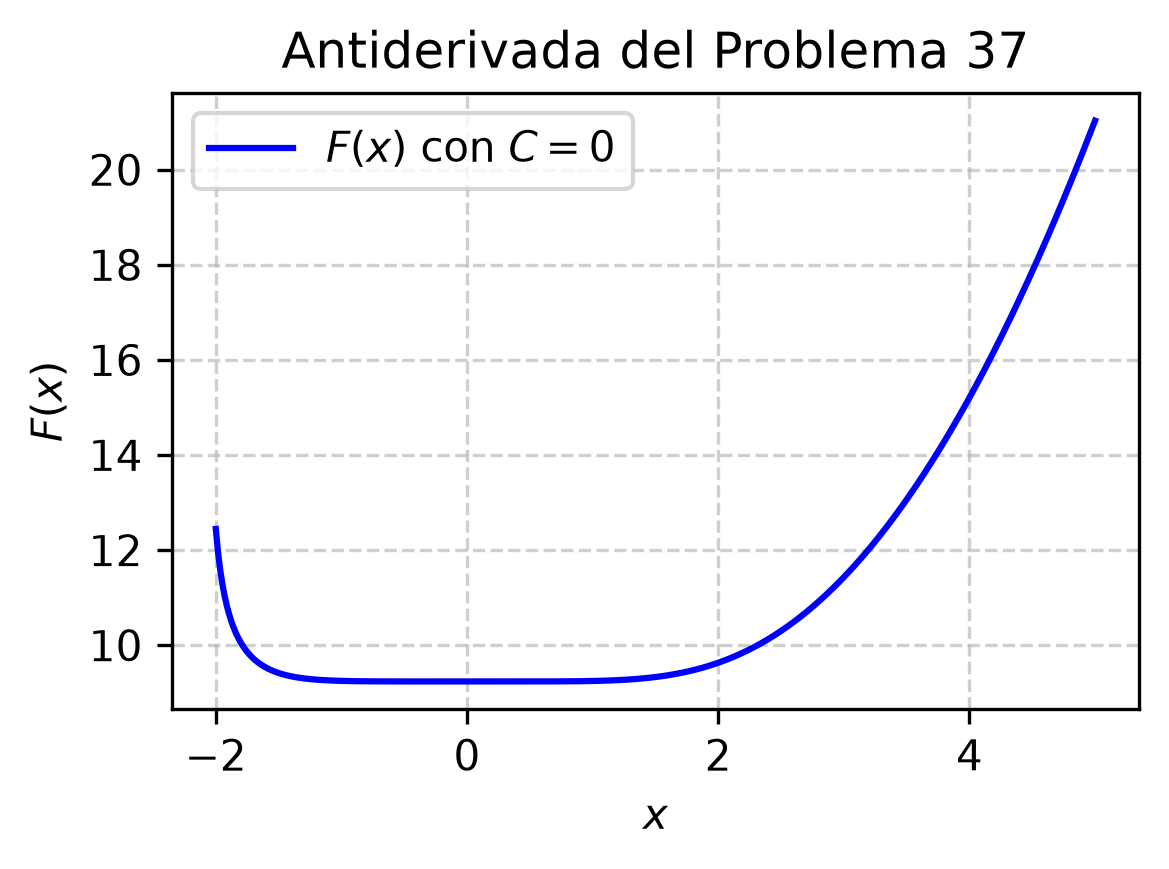
\includegraphics[width=\columnwidth]{semana_05/graficas/SEM05_P37_grafica.png}
	\caption{Representación gráfica de $f(x)$ y su antiderivada $F(x)$ evaluada para la constante de integración $C = 0$ (Problema 37).}
	\label{fig:problema37}
\end{figure}
